In this section, we suppose that 
\begin{itemize}
    \item Graph nodes are natural numebrs.
    \item Every node in a graph has at least one edge.
\end{itemize}
Let $\mathcal{R}$ be finite set of graph relabeling rules.
We establish a mapping $\tau$ that maps graph relabeling rules to term rewriting rules such that there exists a homomorphism from the rewriting relation generated by $\mathcal{R}$ to the rewriting relation on terms generated by $\tau(\mathcal{R})$. We will firstly define the signature and variables of the target term rewriting system, then we will define $\tau$ as a mapping from labeled graphs to terms. Finally, we will extend $\tau$ to graph relabeling rules and state the homomorphism of rewriting relations.

\begin{definition}[Signature and variables of the target term rewriting system]
    The variable set of the target term rewriting system is \(\mathcal{Y} = \{ Y_1, Y_2, \ldots, Y_n \}\). The signature set $\Sigma'$ is defined as the disjoint union of the following sets of symbols:
    \begin{align*}
        \Sigma'_0 &= \Sigma' \cup \{ \text{zero}, \epsilon \}, \\ 
        \Sigma'_1 &= \{\text{succ}, \text{node}\}, \\
        \Sigma'_2 &= \{ \text{edge}, \lambda\}, \\
        \Sigma'_{ac} &= \{ * \},
    \end{align*}
    
    where each symbol in \(\Sigma_k\) has arity \(k\) for all \(k \in \{1,2,3\}\), and the symbols in \(\Sigma_{ac}\) are binary.
    % The set of variables is denoted by \(\chi = \{ Y_1, Y_2, \ldots, Y_n \}\), where
    % \[
    % n \isdef \max \{\text{card}(V(G)) \mid \text{for each rule } r = (G, \lambda, \lambda') \in \mathcal{R}\}
    % \]
    % is the maximum number of nodes present in the graphs of the rules within the relabeling system \(\mathcal{R}\).
    \end{definition}
    \begin{example}
        \label{example_grs_to_trs}
        
        Consider a Graph Relabeling System (GRS) \(\mathcal{R} = \{r\}\) with a unique graph relabeling rule \(r\) depicted as follows:
    
        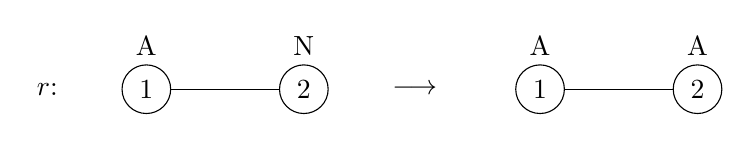
\begin{tikzpicture}
            \draw (-1,0) node[left] {$r$:};
            \node[draw,circle] (x1) at (0,0) {$1$};
            \draw (0,0.3) node[above]{A};
            \node[draw,circle, minimum size = 1pt] (x2) at (2,0) {$2$};
            \draw (2,0.3) node[above]{N};
            \draw[-] (x1) -- (x2);
            
            \draw (3,0) node[right] {$\longrightarrow$};
            
            \node[draw,circle] (x3) at (5,0) {$1$};
            \draw (5,0.3) node[above]{A};
            \node[draw,circle, minimum size = 1pt] (x4) at (7,0) {$2$};
            \draw (7,0.3) node[above]{A};
            \draw[-] (x3) -- (x4);
        \end{tikzpicture}
        
        Given a connected labeled graph \((G, \lambda)\), where all nodes are labeled \(N\) except for one node labeled \(A\), and all edges are labeled \(0\), the set of edges labeled by \(1\) in an \(\mathcal{R}\)-normal labeled graph derived from \((G, \lambda)\) forms a spanning tree of \((G, \lambda)\).
        
        The signature of the corresponding term rewriting system \(\mathcal{R}'\) is defined as \(\Sigma' = \Sigma'_0 \cup \Sigma'_1 \cup \Sigma'_2 \cup \Sigma'_3\), where

        \begin{align*}
            \Sigma'_0 &= \{ N, A, 0, 1, \text{zero} \}, \\
            \Sigma'_1 &= \{ \text{succ}, \text{node} \}, \\
            \Sigma'_2 &= \{ \lambda, \text{edge}, * \},
        \end{align*}
        
        The associative-commutative symbol is denoted by \(\Sigma'_{ac} = \{ * \}\).
    
        The set of variables is \(\chi = \{ Y_1, Y_2 \}\).
        
    \end{example}    

    Since the signature of the term rewriting system is defined, to encode a labeled graph, it suffices to encode its labeling function.

    \begin{definition}[Translation of nodes]
        \label{def:gls_to_actrs:nodes}
        A node \(n\) in a labeled graph is represented by the term $\text{succ}(\text{succ}(\ldots(\text{succ}(\text{zero}))))$.
    \end{definition}

    \begin{definition}[Translation of edges]
        \label{def:gls_to_actrs:edges}
        An arrow $s \overset{l}{\longrightarrow} d$ in a labeled graph is represented by the term $\tau(edge(s', d'), l)$ where $s'$ and $d'$ are the terms representing the nodes $s$ and $d$ respectively.
    \end{definition}
 
\begin{definition}[Translation of graphs]
    \label{def:gls_to_actrs:graphs}
    A labeled graph $G$ is represented by the term $\tau(G)$, which is the concatenation of the terms representing its nodes and edges with the symbol $*$.
\end{definition}
\begin{example}
    The graph  
    \tikz{
            \node[draw,circle] (x1) at (0,0) {$1$};
            \draw (0,0.3) node[above]{A};
            \node[draw,circle, minimum size = 1pt] (x2) at (2,0) {$2$};
            \draw (2,0.3) node[above]{N};
            \draw[-] (x1) -- (x2);
    } is represented by the term 
    $$\lambda(node(succ(zero)),A) * \lambda(node(succ(succ(zero))),N) * \lambda(edge(succ(zero), succ(succ(zero))),0)$$
\end{example}

\begin{example}
    The graph 
    \tikz{
            \node[draw,circle] (x3) at (5,0) {$1$};
            \draw (5,0.3) node[above]{A};
            \node[draw,circle, minimum size = 1pt] (x4) at (7,0) {$2$};
            \draw (7,0.3) node[above]{A};
            \draw[-] (x3) -- (x4);
    } is represented by the term
    $$\lambda(node(succ(zero)),A) * \lambda(node(succ(succ(zero))),A) * \lambda(edge(succ(zero), succ(succ(zero))),1)$$
\end{example}

    % \begin{definition}[Translation of graphs]
    %     \label{def:gls_to_actrs}
    %     Let $(G,\Lambda)$ be a labeled graph.
    %     Let \(\circledast\) be the function that concatenates a set of terms ordered arbitrarily by inserting $*$ between them.

    %     $\tau((G,\Lambda))$ is defined as the term:
    %     \[
    %      \circledast \{ \lambda(\tau(src(e)),\tau(dst(e)),l) \mid 
    %         e \in E(G) \land
    %      \Lambda(e) = l \} 
    %      \]
    %     and $N$ be the term
    %     \[
    %      \circledast \{ \lambda(\tau(n),\Lambda(n)) \mid n \in V(G) \}
    %      \]
    % \end{definition}
     
\textcolor{red}{
    \begin{example}
        Consider the following labeled graph:
        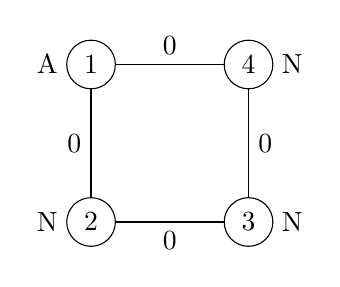
\begin{tikzpicture}
        \draw (1,0) node[above] {0};
        \draw (1,-2) node[below] {0};
        \draw (0,-1) node[left] {0};
        \draw (2,-1) node[right] {0};
        \node[draw,circle] (x_1) at (0,0) {$1$};
        \draw (-0.3,0) node[left]{A};
        \node[draw,circle, minimum size = 1pt] (x_4) at (2,0) {$4$};
        \draw (2.3,0) node[right]{N};
        \node[draw,circle] (x_2) at (0,-2) {$2$};
        \draw (-0.3,-2) node[left]{N};
        \node[draw,circle, minimum size = 1pt] (x_3) at (2,-2) {$3$};
        \draw (2.3,-2) node[right]{N};
        \draw[-] (x_1) -- (x_2);
        \draw[-] (x_2) -- (x_3);
        \draw[-] (x_3) -- (x_4);
        \draw[-] (x_1) -- (x_4);
        \end{tikzpicture}
        This labeled graph is translated into the following term:
        \begin{align*}
            &\lambda(\text{node}(1),A) * \lambda(\text{node}(2),N) * \lambda(\text{node}(3),N) * \lambda(\text{node}(4),N) * \\
            &\lambda(\text{edge}(1,2),0) * \lambda(\text{edge}(2,3),0) * \lambda(\text{edge}(3,4),0) * \lambda(\text{edge}(4,1),0) * \\
            &\lambda(\text{edge}(2,1),0) * \lambda(\text{edge}(3,2),0) * \lambda(\text{edge}(4,3),0) * \lambda(\text{edge}(1,4),0)
        \end{align*}
    \end{example}
}

\begin{definition}[Translation of Graph Relabeling Rule]
    \label{def:gls_to_actrs:rules}
    Let $L \rightarrow R$ be a graph relabeling rule and $L'$ and $R'$ be the terms representing the graphs $L$ and $R$ respectively. The translation of the graph relabeling rule is the term rewriting rule $L'' \rightarrow R''$ where $L''$ and $R''$ are the terms obtained from $L'$ and $R'$, respectively, by replacing every subterm representing a natural number $n$ with the variable $Y_n$.
\end{definition}

    % \begin{definition}[Translation of Graph Relabeling Rule]
    %     A graph relabeling rule $L \to R$ is translated to \(\Gamma(\tau(L)) \to \Gamma(\tau(R)) \), a term rewriting rule with associative-commutative symbol, where the function \(\Gamma\) replaces all occurrences of \(\tau(n)\) with the variable \(Y_n\). 
    % \end{definition}

    \begin{example}
        The rewriting rule 
        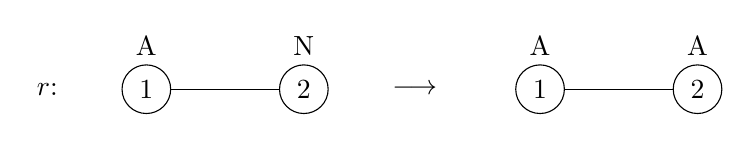
\begin{tikzpicture}
            \draw (-1,0) node[left] {$r$:};
            \node[draw,circle] (x1) at (0,0) {$1$};
            \draw (0,0.3) node[above]{A};
            \node[draw,circle, minimum size = 1pt] (x2) at (2,0) {$2$};
            \draw (2,0.3) node[above]{N};
            \draw[-] (x1) -- (x2);
            
            \draw (3,0) node[right] {$\longrightarrow$};
            
            \node[draw,circle] (x3) at (5,0) {$1$};
            \draw (5,0.3) node[above]{A};
            \node[draw,circle, minimum size = 1pt] (x4) at (7,0) {$2$};
            \draw (7,0.3) node[above]{A};
            \draw[-] (x3) -- (x4);
        \end{tikzpicture}
        is represented by the term rewriting rule $\tau(r)$:
        \begin{align*}
        &\lambda(\opn{node}(Y_1), A) * \lambda(\opn{node}(Y_2), N) * \lambda(\opn{edge}(Y_1,Y_2), 0) * \lambda(\opn{edge}(Y_2,Y_1), 0) \\
        &\longrightarrow \\
        &\lambda(\opn{node}(Y_1), A) * \lambda(\opn{node}(Y_2), A) * \lambda(\opn{edge}(Y_1,Y_2), 1) * \lambda(\opn{edge}(Y_2,Y_1), 1)
    \end{align*}
    \end{example}
    
    %  \begin{lemma}
    %  \label{grs_to_trs_step}
    %  Si $(G, \lambda) \to_{(R, \lambda) \to (R,\lambda'),\varphi}$ est une étape de ré-étiquetage, alors $\overline{(G,\lambda)} \longrightarrow_{\mathcal{R}'} \overline{(G,\lambda')}$.
    %  \end{lemma}
    %  \begin{proof}
    %  Par définition, $m$ est une occurrence de $(G_R,\lambda_R)$ dans $(G,\lambda)$. Par conséquent, $(\varphi(G_R), \lambda_R \circ \varphi^{-1})$ est un sous-graphe de $(G,\lambda)$. Ainsi, $\overline{(\varphi(G_R), \lambda_R \circ \varphi^{-1})}$ est un sous-terme de $\overline{(G,\lambda)}$. Comme le symbole * est associative et commutative, $\overline{(G,\lambda)}$ peut s'écrire $\overline{(\varphi(G),\lambda_R \circ \varphi^{-1})} * A$ où A est un terme de $T(\mathcal{F})$. De même, $\overline{(G,\lambda')}$ peut s'écrire $\overline{(\varphi(G), \lambda_R' \circ \varphi^{-1})} * B$ où B est un terme de $T(\mathcal{F})$. Or on a $A=B$ puis que $\lambda$ et $\lambda'$ ne diffèrent que sur les noeuds et les arêtes du graphe $(G_R,\lambda_{G_R})$.
     
    %  Posons $\sigma = \{(X_v,\varphi(v))\ |\ v\in V(G_R)\}$.  En appliquant la substitution $\sigma$ à la règle $\mathcal{R}^{'}_{R}$, on obtient 
    %  $ \sigma (\overline{\Gamma(\overline{\lambda_R})}) \longrightarrow  \sigma  (\overline{\Gamma (\overline{\lambda_R'})} )$, c'est-à-dire $\overline{(G_R, \lambda_R \circ \varphi^{-1})} \longrightarrow \overline{(G_R, \lambda_R' \circ \varphi^{-1})} $.
     
    %  On en conclut donc $\overline{\lambda} \longrightarrow_{\mathcal{R}'} \overline{\lambda'}$.
    %  \end{proof}
% \begin{lemma}[Preservation of Termination]

% The translation $\tau$ restricted to labeled graphs is a homomorphism, or equivalently : if $(G, \Lambda) \to_{(R, \lambda) \to (R, \Lambda'), \varphi}$ represents a relabeling step, then $\overline{(G,\lambda)} \longrightarrow_{\mathcal{R}'} \overline{(G,\lambda')}$.
% \end{lemma}
\begin{lemma}[Preservation of Termination]
\label{grs_to_trs_step}
Let $\rho = ((R,\lambda) \to (R,\lambda'))$ be a graph relabeling rule. 
Let $(G, \Lambda), (G,\Lambda')$ be two labeled graphs.

If $(G, \Lambda)$ rewrites to $(G, \Lambda')$ using the rule $\rho$, then the term $\tau(G,\Lambda)$ rewrites to the term $\tau(G,\Lambda')$ using the term rewriting rule $\rho' = (\tau(R,\lambda) \to \tau(R,\lambda'))$.
\end{lemma}

\begin{proof}
    Suppose $(G, \Lambda)$ rewrites to $(G, \Lambda')$ using the rule $\rho$. 
    
    By definition, there is a graph isomorphism $m: (R,\lambda) \to (G,\Lambda)$ such that $m(R)$ is a subgraph of $(G,\Lambda)$.
    
    Consequently, $(m(R), \lambda \circ m^{-1})$ is a subgraph of $(G,\Lambda)$. 
    
    Thus, $\tau(m(R), \lambda \circ m^{-1})$ is a subterm of $\tau(G,\Lambda)$. 
    
    Since the symbol $*$ is associative and commutative, we have $$\tau(G,\Lambda) \to_\mathcal{AC}^* \tau(m(R),\lambda \circ m^{-1}) * A$$
    where $A$ is a term. 
    
    Similarly, 
    $$\tau(G,\Lambda')\to_\mathcal{AC}^* \tau(m(R), \lambda' \circ m^{-1}) * B$$
    where $B$ is a term of $T(\mathcal{F})$. 

    Moreover, we have $$A=B$$
    since $\Lambda$ and $\Lambda'$ differ only on the nodes and edges of the unlabeled graph $m(R)$.

    Let $\sigma$ be the substitution which replaces every variable $Y_k$ with $m(k)$, where $k \in V(R)$.
    
    We have 
    $$ \sigma(\opn{lhs}(\rho')) = \tau(m(R), \lambda \circ m^{-1})$$ 
    and  
    $$\sigma(\opn{rhs}(\rho')) = \tau(m(R), \lambda' \circ m^{-1})$$

    Therefore, we conclude that $\tau(m(R),\lambda \circ m^{-1}) * A$ rewrites to $\tau(m(R),\lambda' \circ m^{-1}) * A$ using the term rewriting rule $\rho'$ at position $1$.

    We conclude that $\tau(G,\Lambda)$ rewrites to $\tau(G,\Lambda')$ using the term rewriting rule $\rho'$ in \textbf{ACTRS}.
\end{proof}


% \begin{proof}
% Suppose $(G, \Lambda) \to_{(R, \lambda) \to (R, \lambda'), m} (G, \Lambda)$.

% By definition, $m: (R, \lambda) \to (G, \Lambda)$ is a graph isomorphism. 

% Let $f:E(m(R)) \to \Sigma$ defined by $f(e') = \operatorname{min}_< \set{\Lambda(e)~\mid~e \in E(R)}$ where $\operatorname{min}_<$ return the minimal element in a subset of $\Sigma$. 
% The graph $(m(R), f)$ is a subgraph of $(G, \Lambda)$. Consequently, $\tau(m(G), f)$ is a subterm of $\tau(G, \Lambda)$. Since the symbol * is associative and commutative, $\tau(G, \lambda) \to_\mathcal{AC}^* (m(R), f) * A$, where $A$ is a term in $T(\Sigma',\mathcal{X})$ where $\Sigma'$ is a set of symbols. Similarly, $\tau(G, \Lambda') \to_\mathcal{AC}^*   * B$, where $B$ is a term in $T(\Sigma',\mathcal{X})$. We have $A = B$ because $\Lambda$ and $\Lambda'$ differ only in the nodes and edges of the graph $(R, \lambda)$.
% We have, finally $(m(R), f) * A \to_\rho$
% % Let $\sigma = \{(Y_k, m(k)) \mid k \in V(R)\}$. By applying the substitution $\sigma$ to the rule $\mathcal{R}'_{R}$, we obtain $\sigma (\overline{\Gamma(\overline{\lambda_R})}) \longrightarrow \sigma (\overline{\Gamma (\overline{\lambda_R'})} )$, which simplifies to $\overline{(G_R, \lambda_R \circ m^{-1})} \longrightarrow \overline{(G_R, \lambda_R' \circ m^{-1})}$.

% % Thus, it follows that $\overline{\lambda} \longrightarrow_{\mathcal{R}'} \overline{\lambda'}$.
% \end{proof}


% \begin{lemma}
%     \label{grs_to_trs_sequence}
%     If $(G, \Lambda_0) \to_\mathcal{R} (G, \Lambda_1) 
%         \to_\mathcal{R} \ldots  \to_\mathcal{R}
%         (G, \Lambda_{n-1}) \to_\mathcal{R}
%         (G, \Lambda_n)$ is a relabeling sequence in $\mathcal{R}$, then 
%     $\overline{(G_0, \lambda_0)} \longrightarrow_{\mathcal{R}'} 
%     \overline{(G_1, \lambda_1)} \longrightarrow_{\mathcal{R}'} \ldots 
%     \overline{(G_n, \lambda_n)}$ 
%     is a rewriting sequence in $\mathcal{R}'$.
%     \end{lemma}
    
%     \begin{proof}
%     The proof is by induction on the length of the relabeling sequence, using Lemma \ref{grs_to_trs_step}.
%     \end{proof}
    
    \begin{theorem}
        A graph relabeling system $\mathcal{R}$ terminates, if its translation $\mathcal{R}'$ terminates
    \end{theorem}
    % \begin{proof}
    % The proof is by contradiction, utilizing Lemma \ref{grs_to_trs_sequence}.
    % \end{proof}